\chapter{Software desarrollado} \label{chapter:software}

En este capítulo se describe el software desarrollado para este proyecto. Este software recopila todos los algoritmos de aprendizaje de métricas de distancia analizados en los capítulos anteriores, proporcionando una biblioteca que permite acceder a todos ellos, y con la posibilidad de establecer distintos parámetros que faciliten el aprendizaje. El lenguaje escogido para el desarrollo ha sido Python, aunque también se ha desarrollado un software en R que internamente utiliza la librería anterior.

\section{Los lenguajes Python y R}

\subsection{Python}

Python \cite{python} es un lenguaje de programación de alto nivel, orientado a objetos e interpretado, con tipado dinámico (es decir, las variables pueden tomar valores de distinto tipo a lo largo de la ejecución). Es un lenguaje con una sintaxis sencilla y que dispone de una gran cantidad de librerías que lo han convertido en los últimos años en uno de los lenguajes de programación más populares. Es, en particular, muy popular en el ámbito del aprendizaje automático, al disponer de librerías eficientes dedicadas a este ámbito. El lenguaje está disponible para todas las plataformas, y puede descargarse desde su página web\footnote{\url{https://www.python.org/downloads/}}.

Dentro de las bibliotecas orientadas al aprendizaje automático, la más destacada es Scikit-Learn\footnote{\url{http://scikit-learn.org/stable/}}. Scikit-Learn es una librería de código abierto que proporciona herramientas sencillas y eficientes para distintos campos del aprendizaje automático: clasificación, regresión, clustering, reducción de dimensionalidad, selección de modelos o preprocesamiento. Los algoritmos desarrollados en esta biblioteca siguen las mismas estructuras, lo que los hace fácilmente accesibles. Para utilizar, por ejemplo, un clasificador, en primer lugar se construye un objeto de la clase de dicho clasificador. Durante la construcción se proporcionan los hiperparámetros necesarios para su funcionamiento. Finalmente, basta utilizar el método \texttt{fit} de dicha clase para aprender el clasificador, y con el método \texttt{predict} podemos clasificar nuevos datos. Otro caso que nos resultará de interés son los algoritmos de aprendizaje que trasforman los datos, cuyo funcionamiento es similar al de los clasificadores, en este caso con los métodos \texttt{fit} y \texttt{transform}. Los clasificadores y transformadores son subclases de las clases genéricas \texttt{sklearn.base.ClassifierMixin} y \texttt{sklearn.base.TransformerMixin}, respectivamente, las cuales proporcionan la funcionalidad básica para diseñar nuevos algoritmos de clasificación y transformación. La Figura \ref{fig:ex_clf_trf_python} muestra un ejemplo de su uso.

\begin{figure}[h]
\begin{minted}[
frame=lines,
framesep=2mm,
baselinestretch=1.2,
bgcolor=LightGray,
fontsize=\footnotesize,
linenos
]{python}
    from sklearn.datasets import load_iris # Dataset a utilizar
    from sklearn.neighbors import KNeighborsClassifier # Clasificador k-NN
    from sklearn.preprocessing import MinMaxScaler # Transformación x -> (x-min)/(max - min)

    iris = load_iris()
    X = iris['data']   # Conjunto de datos
    y = iris['target'] # Clases

    # Utilizando el clasificador 3-NN
    knn = KNeighborsClassifier(n_neighbors=3) # Construcción
    knn.fit(X,y) # Aprendizaje
    knn.predict(X[:5,:]) # Asignando clases a los cinco primeros ejemplos.
    # Salida obtenida: array([0, 0, 0, 0, 0])

    # Utilizando MinMaxScaler
    mms = MinMaxScaler() # Construcción
    mms.fit(X) # Aprendizaje
    mms.transform(X[:1,:]) # Transformando el primer dato.
    # Salida obtenida: array([[ 0.22222222,  0.625     ,  0.06779661,  0.04166667]])

\end{minted}
\caption{Uso de los clasificadores y transformadores en Python} \label{fig:ex_clf_trf_python}
\end{figure}


La biblioteca Scikit-Learn está construida sobre el \emph{ecosistema SciPy}\footnote{\url{https://www.scipy.org/}}, un conjunto de bibliotecas de código abierto diseñadas para computación científica, entre las que destacan NumPy\footnote{\url{http://www.numpy.org/}} y la propia librería SciPy, que proporcionan un conjunto de herramientas muy completo para trabajar con vectores, matrices y arrays multidimensionales, la biblioteca Matplotlib\footnote{\url{https://matplotlib.org/}}, para dibujar en 2 dimensiones, y la biblioteca Pandas\footnote{\url{http://pandas.pydata.org/}}, que proporciona estructuras para trabajar con datos y diversos métodos de análisis.

Por último, Python dispone de un repositorio, denominado PyPI\footnote{\url{https://pypi.org/}} (Python Package Index), utilizado para distribuir el software de Python. En este repositorio se pueden encontrar e instalar las bibliotecas más populares de Python, y los desarrolladores de software pueden subir sus paquetes al repositorio. Los paquetes pueden descargarse desde la página web, y también pueden instalarse de forma sencilla desde una línea de comandos (o desde el propio intérprete de Python) utilizando la herramienta \texttt{pip}, la herramienta recomendada para la instalación de paquetes de PyPI. Para la instalación con \texttt{pip}, basta utilizar la sentencia \mintinline{bash}{pip install <nombre_paquete>}.

\subsection{R}

R \cite{R} es un entorno y lenguaje de programación especializado en computación estadística y gráficos. Es también un lenguaje de alto nivel, orientado a objetos, interpretado, con tipado dinámico y diponible en múltiples plataformas. Es de código abierto, y dispone de gran cantidad de bibliotecas en la plataforma CRAN\footnote{\url{https://cran.r-project.org/}} (the Comprehensive R Archive Network) orientadas principalmente al ámbito de la computación estadística.

Además de la computación estadística, R dispone de una gran capacidad para la generación de gráficos, un IDE especializado, RStudio\footnote{\url{https://www.rstudio.com/}} y un lenguaje de documentación basado en LaTeX y Markdown, mediante los cuales es posible elaborar documentos sobre los datos analizados con gran facilidad. También puede integrarse de forma sencilla con lenguajes como C++ o Python. Estas características hacen también a R ser uno de los lenguajes más utilizados para la computación estadística y el aprendizaje automático.

\section{Descripción del software}

Se ha desarrollado una biblioteca para Python, denominada pyDML\footnote{El código de pyDML está disponible en GitHub: \url{https://github.com/jlsuarezdiaz/pyDML}}, que recoge todos los algoritmos estudiados en el capítulo previo. Se ha escogido el lenguaje Python debido a la gran cantidad de herramientas de las que dispone orientadas al aprendizaje automático, como se comentó en la sección anterior, destacando especialmente las operaciones con matrices disponibles en la biblioteca NumPy. Recordemos que la mayoría de técnicas del aprendizaje de métricas de distancia necesitan calcular gradientes de funciones que se aplican sobre matrices, o bien obtener valores y vectores propios de una determinada matriz, o incluso proyectar matrices sobre el cono de las matrices semidefinidas positivas. NumPy dispone de métodos que cubren estas necesidades.

Pero no solo se ha escogido el lenguaje Python por sus herramientas, y es que hasta ahora Python no dispone de una biblioteca completa con algoritmos de aprendizaje de métricas de distancia. En Scikit-Learn es posible encontrar algoritmos como PCA o LDA, englobados dentro de las técnicas de reducción de dimensionalidad de dicha biblioteca, pero algoritmos de aprendizaje de distancias como tales no aparecen. La biblioteca pyDML trata de completar esta carencia de Scikit-Learn.

El diseño seguido para el desarrollo de los algoritmos ha conservado la estructura de los algoritmos de la biblioteca Scikit-Learn. En particular, los algoritmos de aprendizaje de métricas de distancia se incluyen dentro de los algoritmos de transformación, donde la transformación consiste justamente en aplicar a los datos la aplicación lineal aprendida. Por ello, se ha optado por implementar los distintos algoritmos como subclases de \texttt{sklearn.base.TransformerMixin}. Adicionalmente, los algoritmos de aprendizaje de métricas de distancia aportan una métrica (excepto los basados en kernels) y una transformación lineal (ambas son recuperables a partir de la otra, aunque cada algoritmo aprenda solo una de las dos opciones). Será importante poder tener acceso a ellas para el cálculo de distancias, por lo que todos los algoritmos de aprendizaje de métricas implementarán, además de los métodos \texttt{fit} y \texttt{transform}, los métodos \texttt{metric} y \texttt{transformer}, que darán acceso a estos elementos.

Por ello, en el diseño final se ha implementado la clase abstracta \texttt{DML\_Algorithm}, que proporciona las funcionalidades comunes a todos los algoritmos de aprendizaje de métricas de distancia, esto es, da acceso a las matrices aprendidas mediante los métodos \texttt{metric()} y \texttt{transformer()}, y define la función \texttt{transform(X)}, la cual devuelve el conjunto de datos resultante de aplicar la transformación aprendida a cada dato de \texttt{X}. Adicionalmente se incluye el método \texttt{metadata()}, que proporciona información adicional sobre lo aprendido por cada algoritmo, útil a la hora de estimar parámetros. Cada uno de los algoritmos de aprendizaje de métricas de distancia forma una subclase de \texttt{DML\_Algorithm} implementando un método \texttt{fit(X,y)} propio encargado de aprender la distancia a partir de los datos etiquetados dados por \texttt{X} e \texttt{y}. Para el caso de los algoritmos basados en kernels se ha creado una subclase de \texttt{DML\_Algorithm}, \texttt{KernelDML\_Algorithm}, que aporta las funcionalidades específicas de los kernels (Figura \ref{fig:diag_clases_pyDML}). 

\begin{figure} 
    \centering
    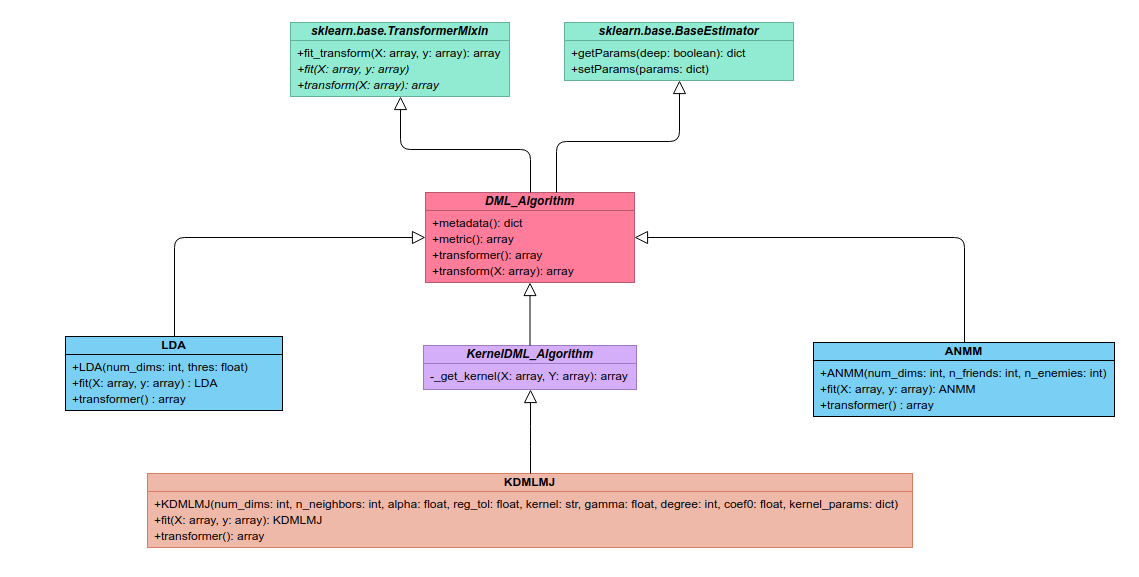
\includegraphics[width=0.75\textwidth]{images/uml_pydml.png}
    \caption{Diagrama de clases de los algoritmos desarrollados en pyDML (se muestran solo los algoritmos LDA, ANMM y KDMLMJ, pero el resto de algoritmos sigue una estructura análoga, sobreescribiendo el método \texttt{metric()} o \texttt{transformer()} según la forma de aprender del algoritmo).} \label{fig:diag_clases_pyDML}
\end{figure}

Es importante destacar, para finalizar la descripción de los algoritmos, que estos incluyen distintos hiperparámetros que se pueden modificar para mejorar la ejecución o cambiar las condiciones de las distancias aprendidas. Estos parámetros varían con cada algoritmo, y los más comunes y de mayor importancia en la ejecución de los algoritmos son:
\begin{itemize}
    \item \textbf{Número de dimensiones.} Dimensión deseada para la transformación a aprender. Está presente en todos los algoritmos de reducción de dimensionalidad, aunque la mayoría de los algoritmos que aprenden aplicaciones lineales admiten este parámetro.
    \item \textbf{Número de vecinos.} Los parámetros de este tipo determinan cuántos datos se eligen para la construcción de vecindarios en los algoritmos que realizan estas construcciones, como es el caso de ANMM, LMNN o DMLMJ.
    \item \textbf{Método de descenso o algoritmo de resolución.} En los algoritmos que minimizan una función diferenciable puede establecerse el método de descenso deseado. Entre las opciones válidas, que dependerán del algoritmo y de las restricciones de la función, destacan el gradiente descendente clásico (BGD), el gradiente descendente estocástico (SGD, una variante del primero donde la regla de adaptación se aplica dato por dato, en lugar de considerar todo el gradiente; la dirección esperada final sigue siendo la del gradiente y suele proporcionar mejores resultados) o la programación semidefinida (SDP) consistente en gradiente descendente con proyecciones sobre el cono de las matrices semidefinidas positivas.
    \item \textbf{Tasa de aprendizaje.} En los algoritmos basados en gradiente descendente, se puede establecer un valor inicial para la tasa de aprendizaje, y cómo varía esta: constante, o adaptiva. En el último caso, si la iteración del gradiente a mejorado el valor de la función objetivo, la tasa se incrementa. En caso contrario, se reduce. Los factores de aumento y reducción también son parámetros que se pueden establecer.
    \item \textbf{Criterios de parada.} En los algoritmos basados en gradiente descendente, es necesario establecer criterios de parada. Los criterios disponibles en la mayoría de algoritmos consisten en número máximo de iteraciones, precisión (cercanía de la norma del gradiente al valor nulo) o tolerancia (diferencia entre dos iteraciones del gradiente).
    \item \textbf{Parámetros de regularización.} Algunos algoritmos requieren parámetros de regularización para, por ejemplo, evitar matrices singulares (la proposición \ref{prop:pd_regularization} nos dice cómo utilizar estos parámetros). Tanto los parámetros de regularización como los criterios que determinan su aplicación pueden establecerse en los algoritmos que lo requieran.
\end{itemize}
Una descripción detallada de todos los hiperparámetros para cada algoritmo puede consultarse en la documentación oficial\footnote{\url{https://pydml.readthedocs.io/} \label{pydml_doc_url}}.

Adicionalmente a los algoritmos de aprendizaje, se han desarrollado dos clasificadores basados en distancias, también siguiendo la estructura de Scikit-Learn. El primero de ellos es un wrapper para el clasificador de vecinos cercanos proporcionado en Scikit-Learn, de forma que pueda actuar conjuntamente con un algoritmo de aprendizaje de métricas de distancia, lo cual hasta ahora no era posible hacer directamente con el clasificador de vecinos cercanos de Scikit-Learn. Por otro lado, se ha añadido el clasificador de múltiples centroides, mediante la clase \texttt{NCMC\_Classifier}. Actualmente Scikit-Learn solo dispone de clasificador NCM de la media más cercana\footnote{Véase \url{http://scikit-learn.org/stable/modules/generated/sklearn.neighbors.NearestCentroid.html}}. \texttt{NCMC\_Classifier} añade la posibilidad de añadir más de un centroide por clase, y así puede ser optimizado por el algoritmo de aprendizaje de distancias NCMC.

Por último, la librería pyDML también incorpora herramientas gráficas para la representación y evaluación de las distancias aprendidas, las cuales utilizan internamente la librería Matplotlib. Las funciones incorporadas permiten representar datos etiquetados, junto a las regiones determinadas por cualquier clasificador de Scikit-Learn (\texttt{classifier\_plot}). También permite comprobar cómo cambia la región determinada por un clasificador basado en distancias si cambiamos la distancia (\texttt{dml\_plot}). Una función especializada facilita el dibujo de regiones para el clasificador k-NN (\texttt{knn\_plot}). De la misma forma, se añaden funciones para representar distintos pares de atributos, junto con una sección de la región del clasificador, para conjuntos de datos de mayores dimensiones (\texttt{classifier\_pairplots}, \texttt{dml\_pairplots}, \texttt{knn\_pairplots}). Por último, múltiples dibujos comparando distintos clasificadores o distancias también pueden elaborarse, gracias a la función \texttt{dml\_multiplot}. La descripción detallada de estas funciones y sus argumentos puede consultarse de nuevo en la documentación\cref{pydml_doc_url}. En ella también pueden consultarse los parámetros de las funciones \texttt{tune}, la última funcionalidad adicional incorporada, que permite estimar los parámetros de los algoritmos de aprendizaje de distancias mediante validación cruzada, utilizando como medidas la tasa de acierto de clasificadores k-NN o alguno de los metadatos de los algoritmos.

Para el lenguaje R se ha desarrollado la biblioteca rDML\footnote{El código de rDML está disponible en GitHub: \url{https://github.com/jlsuarezdiaz/rDML}}, la cual contiene funciones que actúan de wrapper para las distintas funcionalidades implementadas en pyDML. Es, por tanto, una biblioteca que aporta las mismas funcionalidades del aprendizaje de métricas de distancia para el lenguaje R. De nuevo, la elección de R se debe a sus características como lenguaje orientado al aprendizaje automático, y a que tampoco hay presente una librería amplia con algoritmos de aprendizaje de métricas de distancia. La integración con Python se ha realizado de forma sencilla gracias a la biblioteca \texttt{reticulate}\footnote{\url{https://rstudio.github.io/reticulate/articles/introduction.html}} de R.


\section{Uso del software}

La instalación de la biblioteca pyDML puede realizarse a través de PyPI, utilizando la orden \texttt{pip install pyDML}. También es posible descargar o clonar directamente el repositorio desde GitHub. En tal caso, la instalación del software puede realizarse ejecutando el script de configuración disponible en el directorio raíz, mediante la orden \mintinline{bash}{python setup.py install}. Una vez instalado, podemos acceder a todos los algoritmos de aprendizaje de métricas de distancia, y a las funcionalidades adicionales importando la clase que deseemos dentro del módulo \texttt{dml}.

Como ya hemos dicho, la forma de uso de los algoritmos de aprendizaje de distancias es análoga a la de los algoritmos de transformación de Scikit-Learn. En la Figura \ref{fig:ex_dml} se muestra un ejemplo para el caso del algoritmo NCA. Con el resto de algoritmos el funcionamiento es el mismo, variando posiblemente los distintos hiperparámetros.

\begin{figure}[h]
\begin{minted}[
frame=lines,
framesep=2mm,
baselinestretch=1.2,
bgcolor=LightGray,
fontsize=\footnotesize,
linenos
]{python}
    >>> import numpy as np # Biblioteca NumPy
    >>> from sklearn.datasets import iris # Iris dataset

    >>> from dml import NCA # Importamos el algoritmo NCA

    >>> iris = load_iris() # Cargamos los datos de iris
    >>> X = iris['data']
    >>> y = iris['target']

    >>> nca = NCA()  # Construcción del algoritmo (con parámetros por defecto)
    >>> nca.fit(X,y) # Aprendemos la distancia con fit.

    >>> nca.metadata() # Podemos consultar los metadatos asociados al algoritmo
    {'final_expectance': 0.95771240234375,
     'initial_expectance': 0.8380491129557291,
     'num_iters': 3}

    >>> nca.metric() # También podemos ver la métrica aprendida
    array([[ 1.19098678,  0.51293714, -2.15818151, -2.01464351],
           [ 0.51293714,  1.58128238, -2.14573777, -2.10714773],
           [-2.15818151, -2.14573777,  6.46881853,  5.86280474],
           [-2.01464351, -2.10714773,  5.86280474,  6.83271473]])

    >>> nca.transformer() # o la aplicación lineal asociada.
    array([[ 0.77961001, -0.01911998, -0.35862791, -0.23992861],
           [-0.04442949,  1.00747788, -0.29936559, -0.25812144],
           [-0.60744415, -0.57288453,  2.16095076,  1.35212555],
           [-0.46068713, -0.48755353,  1.25732916,  2.20913531]])

    >>> # Por último, podemos transformar los datos según la aplicación aprendida
    >>> Lx = nca.transform()
    >>> Lx[:5,:] # Los 5 primeros datos transformados
    array([[ 3.35902632,  2.8288461 , -1.80730485, -1.85385382],
           [ 3.21266431,  2.33399305, -1.39937375, -1.51793964],
           [ 3.0887811 ,  2.57431109, -1.60855691, -1.64904583],
           [ 2.94100652,  2.41813313, -1.05833389, -1.30275593],
           [ 3.27915332,  2.93403684, -1.80384889, -1.85654046]])

    >>> # O también podemos transformar nuevos datos
    >>> X_ = np.array([[1.0,0.0,0.0,0.0],[1.0,1.0,0.0,0.0],[1.0,1.0,1.0,0.0]])
    >>> Lx_ = nca.transform(X_)
    >>> Lx_
    array([[ 0.77961001, -0.04442949, -0.60744415, -0.46068713],
           [ 0.76049003,  0.9630484 , -1.18032868, -0.94824066],
           [ 0.40186212,  0.66368281,  0.98062208,  0.3090885 ]])

\end{minted}
\caption{Uso de los algoritmos de aprendizaje de métricas de distancia en pyDML} \label{fig:ex_dml}
\end{figure}

El uso de los clasificadores de la biblioteca es análogo al mostrado en el ejemplo de la Figura \ref{fig:ex_clf_trf_python}. En cuanto a las funciones de dibujado, se muestra un ejemplo en la Figura \ref{fig:ex_dmlplot}. En la documentación\footnote{\url{https://pydml.readthedocs.io/en/latest/examples.html}} pueden consultarse ejemplos más detallados sobre todas las posibilidades que ofrece pyDML.

\begin{figure}[h]
\begin{minted}[
frame=lines,
framesep=2mm,
baselinestretch=1.2,
bgcolor=LightGray,
fontsize=\footnotesize,
linenos
]{python}
    >>> import numpy as np
    >>> from sklearn.datasets import load_iris
    >>> from dml import NCA, LDA, NCMC_Classifier, dml_multiplot

    >>> iris = load_iris()
    >>> X = iris['data']
    >>> y = iris['target']

    >>> # Inicializamos los algoritmos de aprendizaje
    >>> nca = NCA()
    >>> lda = LDA()
    >>> ncmc = NCMC()

    >>> # Vamos a ver cómo cambian los clasificadores 3-NN y NCMC aprendiendo una distancia previamente
    >>> # Dibujaremos 4 figuras: {NCMC, NCMC+NCA, 3-NN, 3-NN+LDA}
    >>> # NCMC lo añadimos como parámetro en la lista de clasificadores (clfs)
    >>> # 3-NN lo añadimos como parámetro en la lista de vecinos (ks)
    >>> # LDA y NCA lo añadimos en la lista de algoritmos de aprendizaje de distancias (dmls)
    >>> # No queremos transformar los datos, sino ver cómo cambia la región (transforms)
    >>> dml_multiplot(X[:,[0,1]],y,nrow=2,ncol=2,ks=[None,None,3,3],
    >>>               clfs=[ncmc,ncmc,None,None],dmls=[None,nca,None,lda],
    >>>               transforms=[False,False,False,False],title="Comparing",
    >>>               subtitles=["NCMC","NCMC + NCA","3-NN","3-NN + LDA"],
    >>>               cmap="rainbow",figsize=(12,12))
\end{minted}
\\
\centering
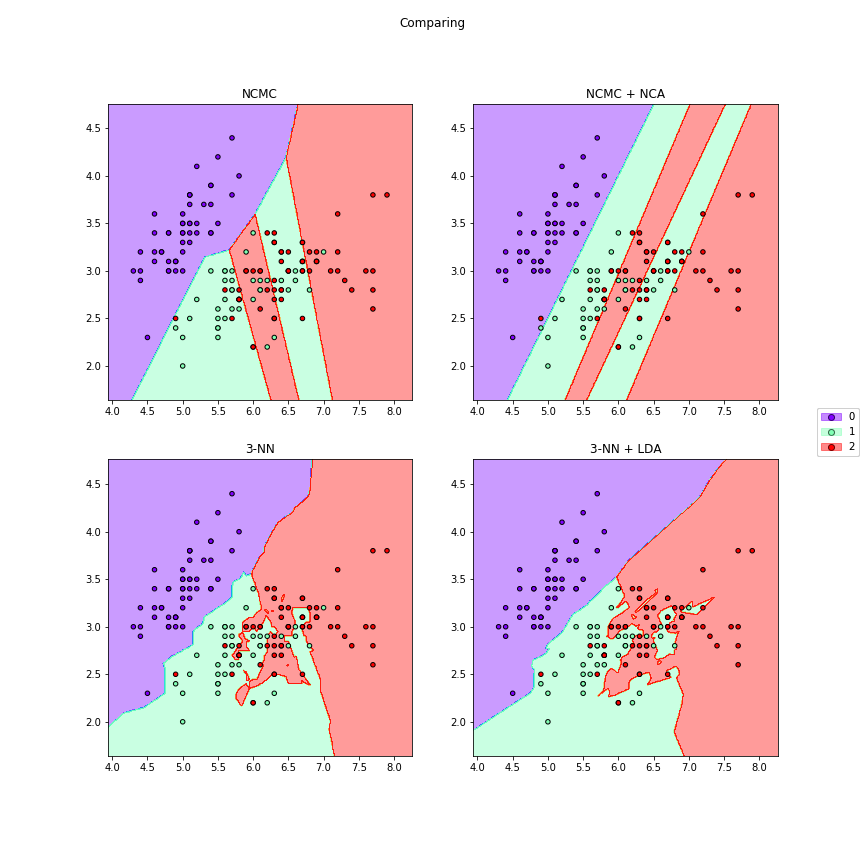
\includegraphics[width=0.7\textwidth]{images/plotdoc7.png}

\caption{Dibujo de clasificadores basados en distancias con pyDML} \label{fig:ex_dmlplot}
\end{figure}

En cuanto a la biblioteca rDML, la instalación puede realizarse a través del paquete \texttt{devtools}, ejecutando en la terminal de R el comando
\begin{minted}{r}
    devtools::install_github("jlsuarezdiaz/rDML")
\end{minted}
Una vez instalado, podemos cargar la biblioteca mediante la orden
\begin{minted}{r}
    library(rDML)
\end{minted}
La biblioteca rDML proporciona un conjunto de variables en forma de listas que contienen las distintas funcionalidades implementadas, agrupadas según el cometido que realizan. Así, la variable fundamental es la denominada \texttt{dml}, mediante la cual podemos acceder a todos los algoritmos de aprendizaje de métricas de distancia (por ejemplo, para NCA, \texttt{dml\$NCA()}). Cada una de estas funciones inicializa una lista cuyos distintos elementos son las funciones del algoritmo asociado de pyDML. A dichas funciones podemos acceder por su nombre, pudiendo de esta forma trabajar de forma a análoga a la realizada en pyDML. De la misma forma, las listas \texttt{distance\_clf}, \texttt{dml\_plotter} y \texttt{dml\_tune} permiten acceder a los clasificadores de pyDML, a las funciones de dibujo y a las funciones de estimación de parámetros, respectivamente. La Figura \ref{fig:ex_dml_r} muestra el ejemplo de la Figura \ref{fig:ex_dml} adaptado a R. Una variedad más amplia de ejemplos puede consultarse en la documentación\footnote{\url{https://jlsuarezdiaz.github.io/software/rDML/docs/}}.
\begin{figure}[h]
\begin{minted}[
frame=lines,
framesep=2mm,
baselinestretch=1.2,
bgcolor=LightGray,
fontsize=\footnotesize,
linenos
]{r}
    >>> library(datasets)
    >>> library(rDML)
    
    >>> data(iris) # Dataset iris
    >>> X = iris[1:4]
    >>> y = iris[5][,1]
    
    >>> nca = dml$NCA() # Inicialización del algoritmo de aprendizaje.
    >>> nca$fit(X,y) # Aprendiendo la distancia.
    
    >>> nca$metadata() # Metadatos del algoritmo
    $num_iters
    [1] 1
    $initial_expectance
    [1] 0,8380717
    $final_expectance
    [1] 0,9470497
    
    >>> nca$metric() # Podemos ver la métrica aprendida
               [,1]       [,2]      [,3]       [,4]
    [1,]  1,1880811  0,2666971 -1,187263 -1,0341494
    [2,]  0,2666971  1,2597098 -1,093658 -0,9961411
    [3,] -1,1872632 -1,0936585  4,319512  3,1971420
    [4,] -1,0341494 -0,9961411  3,197142  3,9139584
    
    >>> nca$transformer() #También podemos ver la aplicación lineal aprendida
               [,1]        [,2]       [,3]       [,4]
    [1,]  0,9751869  0,02021321 -0,2213029 -0,1632234
    [2,]  0,0398954  1,03907054 -0,2488276 -0,2153292
    [3,] -0,3782439 -0,32006211  1,8775001  0,8850434
    [4,] -0,3040256 -0,27783779  0,8268102  1,7486132
    
    >>> Lx = nca$transform() # Finalmente podemos obtener los datos transformados
    >>> Lx[1:5,]
             [,1]     [,2]         [,3]       [,4]
    [1,] 4,701731 3,448789 -0,243752362 -1,0157060
    [2,] 4,496587 2,921275 -0,008072532 -0,8159819
    [3,] 4,327722 3,145992 -0,184186187 -0,8934254
    [4,] 4,183922 2,988330  0,261144437 -0,6698770
    [5,] 4,606233 3,548706 -0,237934184 -1,0130872
    
    >>> # O transformar nuevos datos
    >>> X_ = matrix(nrow = 3, ncol = 4, data = c(1,0,0,0,  1,1,0,0,  1,1,1,0))
    >>> Lx_ = nca$transform(X_)
    >>> Lx_
               [,1]       [,2]      [,3]      [,4]
    [1,]  0,8119635 -0,1754338 0,5067995 1,4445876
    [2,] -0,1430102  0,8237414 0,5649813 1,4707754
    [3,] -0,2010897  0,7902429 1,5574380 0,5489725
\end{minted}

\caption{Uso de los algoritmos de aprendizaje de métricas de distancia en rDML} \label{fig:ex_dml_r}
\end{figure}